\chapter{引言}\label{chap:introduction}

\section{背景}

随着信息技术的飞速发展，数据安全问题已成为全球关注的焦点。端到端加密通信协议作为保障信息传输安全的重要技术手段，广泛应用于即时通讯、电子支付、远程办公等领域。通过对通信内容进行加密，端到端加密协议能够有效保护数据的机密性和完整性，防止信息在传输过程中被窃取或篡改，确保通信双方的隐私安全。


早期的即时通信协议通常缺乏足够的安全性，甚至几乎没有安全保障。例如，一些系统虽然在用户设备与服务提供商的服务器之间使用了加密技术，但仍然使得服务提供商能够在消息从一个用户转发到另一个用户的过程中查看消息的明文。PGP加密电子邮件\cite{zimmermann1995official}为用户提供了实现端到端加密通信的一种方式，但其可用性问题意味着无法面向广大的普通用户。显然，我们需要一种全面安全的端到端加密技术，以保护即时通讯免受攻击者的威胁，尤其是潜在的恶意服务提供商。

在过去十年中，通信协议的安全性已经取得了显著进展。Off-the-Record Messaging Protocol (OTR) \cite{borisov2004off} 是最早为双方即时通讯提供端到端安全性的协议之一，主要通过插件或附加组件的形式将加解密功能集成到现有的即时通讯客户端中使用。由于聊天会话可能是长期持续的，并且在会话持续的长时间内，用户设备可能会在某个时间点被攻破。因此，OTR 协议在每次聊天消息的往返过程中都会进行一次新的 Diffie-Hellman (DH) 密钥交换，以生成新的消息密钥。现在这种技术我们称之为非对称棘轮（Asymmetric Ratchet），它使得攻击者即使在某一个时间点攻破了设备，也难以计算未来的消息加密密钥。

虽然 OTR 并未得到广泛采用，但它对 Signal 协议 \cite{signal_docs} 的设计产生了深远影响。Signal 协议由 Marlinspike 和 Perrin 开发，结合了隐式认证的密钥交换协议和棘轮机制，实现了具有真实性、可否认性以及前向安全和后向安全等多种安全属性的端到端加密消息传输。Signal 协议在实现端到端加密的同时，并未牺牲异步性：消息可以通过中继服务器在任何时间从发送方发送到接收方，而接收方无需在线即可完成密钥交换。Signal 协议不仅在同名应用 Signal Messenger 中得到了广泛应用，还被 WhatsApp、Facebook Messenger等国际通信软件采纳，成为当前最主流的端到端加密标准之一。

然而，随着量子计算技术的快速发展，传统加密算法正面临前所未有的挑战。 当前广泛使用的公钥加密体制，如基于 DH 密钥交换和椭圆曲线密码学(ECC)的算法，其安全性依赖于大整数分解或离散对数等数学难题。而这些难题在理论上可以被足够强大的量子计算机利用 Shor 算法\cite{shor1994algorithms}高效求解。一旦实用化的量子计算机问世，现有的端到端加密协议将面临被彻底破解的风险，导致历史通信记录和未来通信内容均可能暴露。


综上所述，端到端加密通信不仅是应对当前网络威胁的必要手段，更需面向未来，发展具备后量子能力的安全协议，以应对下未来量子计算机带来的根本性挑战。


\section{国内外研究现状}\label{sec:system}

\subsection{传统端到端加密通信协议}

传统端到端加密协议中，OTR 和 Signal 是两个具有代表性的方案。
 
OTR 协议于 2004 年提出，旨在为即时通信提供加密保护和可否认性，即通信双方无法向第三方证明对话内容。它通过 DH 密钥交换实现前向安全，并采用棘轮机制动态更新密钥，防止长期密钥泄露后历史消息被解密。然而，OTR 要求通信双方必须同时在线，不支持异步消息收发，也无法实现后向安全。此外，其依赖手动密钥验证，使用复杂，缺乏商业推广，最终未能广泛普及。更重要的是，其核心加密机制基于传统公钥算法，无法抵御未来的量子攻击。

Signal 协议在 OTR 基础上实现了显著改进。它采用 Extended Triple Diffie-Hellman (X3DH)\cite{marlinspike2016x3dh} 协议完成安全密钥协商，并引入双棘轮机制\cite{alwen2019double}，在每次消息交互中更新密钥，不仅强化了前向安全，还实现了后向安全。同时，Signal 支持异步通信，用户无需同时在线即可安全收发消息，极大提升了实用性。正因如此，该协议被 WhatsApp 等主流应用广泛采用。

尽管 Signal 协议在安全性与可用性上表现优异，但它仍依赖椭圆曲线等传统公钥密码算法。这些算法在量子计算机面前存在被破解的风险。随着量子计算的发展，OTR 和 Signal 等现有协议都将面临根本性威胁，亟需向后量子密码体系演进。






\subsection{后量子端到端加密通信协议}

考虑到系统的性能、兼容性以及平稳过渡性，一些研究选择以混合模式融入后量子密码学，即同时使用现有的经典算法和后量子算法，以确保只要其中一种算法未被破解，通信就是安全的。因此，在许多情况下，为了使现有通信协议具备后量子安全性，人们选择混合模式融入后量子密码技术，目前，这种方法正在被考虑应用于多种协议，包括 TLS\cite{stebila2023hybrid} 和 SSH\cite{kampanakis2023ssh}。同时，这种混合模式正在被用于端到端加密协议中，包括 Signal 升级版 Signal-PQXDH 协议\cite{kret2023pqxdh} 和 苹果公司的PQ3协议\cite{stebila2024security}。

\textbf{1. Signal-PQXDH协议}


Signal 在2023年初将其 X3DH 规范升级为Post-Quantum Extended Diffie-Hellman（PQXDH）协议。PQXDH 在之前的 X3DH 握手基础上增加了后量子 KEM 组件，采用的是一种混合模式。PQXDH协议初始化阶段公私钥对生成基于curve25519算法\cite{bernstein2006curve25519}和CRYSTALS-Kyber (Kyber) \cite{kyber2022}密钥封装机制，后续密钥更新基于curve25519算法，数字签名仍然采用XEdDSA算法\cite{perrin2016xeddsa}。

% \begin{figure}[ht]
%     \centering
%     \includegraphics[width=1\linewidth]{毕设/开题报告/Img/PQXDH.png}
%     \caption{PQXDH协议初始化阶段基本流程}
%     \label{fig:enter-label}
% \end{figure}

PQXDH 协议初始化包含以下三个主要阶段：
\begin{itemize}
    \item 密钥发布：Bob 将他的椭圆曲线身份密钥、预密钥和后量子密钥封装密钥的公钥上传到服务器。
    \item 发送初始消息：Alice 从服务器获取 Bob 的预密钥包，并使用这些密钥和自己的私钥通过 DH 和 Hash 运算得到共享密钥，同时发送加密的初始消息。
    \item 接收初始消息：Bob 接收并处理 Alice 的初始消息，完成密钥协商。
\end{itemize}

% 目前，后量子 Signal 协议已在 Signal 客户端的最新版本中实现并投入使用。新聊天会在双方使用最新 Signal 软件后默认使用 PQXDH 协议，同时Signal 团队也计划逐步禁用 X3DH，要求所有新聊天均使用 PQXDH 协议，以保护语音和文本消息免受量子计算机攻击。PQXDH相比X3DH多了一个后量子组件，用于密钥初始化阶段。

PQXDH协议在初始阶段结合了传统ECDH\cite{haakegaard2015elliptic}和后量子密钥封装机制（PQKEM），给初始密钥协商阶段提供了后量子属性，增强了初始阶段的量子安全性。然而，后续用于密钥更新的双棘轮机制仍基于经典椭圆曲线密码算法，后续密钥更新阶段仍存在量子威胁：对称棘轮使用基于hmac\cite{krawczyk1997hmac}的密钥导出函数（HKDF \cite{Kra10}）来更新密钥，非对称棘轮依赖ECDH进行密钥交换，均未集成后量子组件。因此，尽管协议具有前向安全性和后向安全性，但这些属性在量子攻击下很难成立。如果后续的 ECDH 密钥交换被量子计算机破解，那么对于该根密钥下的未来会话将不再安全。





\textbf{2. PQ3协议}

苹果公司于2024年2月份发表了PQ3协议，PQ3是一种更安全的具备后量子安全的端到端通信加密协议，代表了端到端通信加密技术的前沿。
 
PQ3在非对称棘轮阶段引入了后量子密钥封装算法Kyber\cite{bos2018crystals}，并与经典ECDH结合，形成混合的后量子密钥协商。这使得即使未来量子计算机出现，攻击者也难以破解通信密钥，从而实现了后量子的前向安全和后向安全。

然而，为了控制带宽开销和提升性能，PQ3协议并非每次消息都进行非对称棘轮更新，而是由上层应用设定在会话中每发送约50条消息或间隔一周时，才进行一次完整的非对称棘轮密钥更新。这意味着在两次更新之间，会话长期处于同一根密钥阶段。如果在此期间设备被攻破，攻击者可能获取当前密钥状态，从而解密该阶段内所有消息，这在一定程度上削弱了前向安全的强度，延长了密钥暴露的窗口期。


综上，PQ3通过将后量子密钥封装算法集成到双棘轮机制中，显著提升了长期通信的抵抗后量子攻击的能力。但其较长的根密钥更新周期在降低密钥计算开销和带宽消耗的同时，也带来了阶段性安全强度下降的风险。

\subsection{关键问题}
目前，许多流行的通讯应用，如Signal、WhatsApp、Telegram和苹果的iMessage等，均采用了端到端加密技术。2024年，微信也宣布将加强其聊天加密技术，采用端到端加密和双重认证来提升用户数据的安全性。
然而，随着量子计算机的发展，传统的端到端加密通信协议的公钥密码学基础难题正面临被攻破的威胁，虽然国际上已有一些端到端加密通信的后量子迁移研究，但目前端到端加密通信协议的研究还存在以下问题：


\subsubsection{后量子加密通信带来的开销问题}

为了应对量子计算机和量子算法带来的威胁，学术界提出了多种基于数学难题的密码学算法，这些难题无法通过 Shor 的量子算法解决。NIST 宣布启动后量子密码学标准化项目，目标是标准化后量子的公钥加密或密钥封装机制（KEMs）以及数字签名方案。经过多年的多轮评审，NIST 于 2022 年宣布了四种后量子算法的标准化结果：密钥封装机制 CRYSTALS-Kyber\cite{bos2018crystals} ，以及三种数字签名方案（CRYSTALS-Dilithium \cite{lyubashevsky2020crystals}、Falcon\cite{prest2020falcon}  和 SPHINCS+\cite{bernstein2019sphincs+}）。


基于这些标准化的后量子密码算法成果，学术界和工业界开始更新和重新设计通信协议，在原先协议中加入后量子组件，进行后量子升级。虽然后量子密码算法已经标准化，但是从经典密码向后量子密码学的过渡并不简单。其中一个原因是，现有的后量子算法通常比传统算法的通信开销更大。从根密钥更新的角度来看， 一次根密钥更新需要传输 后量子公钥（1184B）和密文（1088B），带宽消耗为 2278 字节，而传统端到端加密通信协议 Signal 进行一次根密钥更新仅需 32 字节，两者相差了将近70倍。从用户体验角度来看，这会显著增加通信的延迟，从工程角度来看，这将大幅提高带宽、存储和能耗成本。另外一个原因是非对称棘轮的计算开销较大：每次更新都需要同时执行  (ECDH) 和 后量子 KEM 的封装或解封操作。这些非对称运算涉及大整数运算与多项式变换，在资源受限的移动设备上，这种额外的计算负担会带来 显著的 CPU 占用、能耗增加和更高的通信延迟。

所以，如何优化后量子升级带来的计算和带宽消耗问题，是我们亟需解决的问题。


\subsubsection{ 国内端到端加密通信协议后量子迁移研究不够深入}

目前，我国在端到端加密通信协议的后量子研究方面还存在空白，具体表现为尚未发现相关的研究发表在国内或国际的学术（会议）期刊上，也不存在落地的端到端通信加密应用。

尽管我国在后量子密码领域已取得显著研究成果，如 Aigis-Enc\cite{Shen2021AigisEnc}、CTRU/CNTR\cite{Zheng2024NTRU}、Sphincs-Alpha\cite{zhang2022sphincs}、Aigis-Sig\cite{PQMagic} 等自主设计的密钥封装与签名方案，部分算法进入国际评测视野，但整体上仍缺乏统一的国家或行业标准体系，标准化进程相对滞后于NIST主导的国际步伐。

相比之下，欧美已在积极推动后量子密码在通信协议中的落地：如 Signal 协议已经升级为 PQXDH，苹果公司推出 PQ3 协议，具备多阶段后量子前向与后向安全。而国内主流通信平台如微信、QQ 虽在2024年宣布加密升级，但其机制仍为传输层或服务器端加密，未实现端到端加密，在此类架构下，服务提供商仍具备明文数据的访问权限，难以满足高敏感信息传输场景对长期保密性的需求，尤其无法抵御未来量子计算技术成熟后可能出现的 “先窃取、后解密”（harvest-now, decrypt-later）攻击风险，对信息安全构成潜在威胁。

因此，开展面向自主可控目标的后量子端到端加密协议研究，具有重要的理论价值与现实意义。该研究不仅能够有效提升我国在网络安全领域的核心技术竞争力，更为构建分层级、可扩展且兼顾安全性与合规性的新型通信基础设施提供关键技术支撑。从应用场景优先级来看，此类研究可优先聚焦政务、金融、科研等对信息长期保密性要求较高的专用领域，在严格保障国家信息安全的前提下，探索实现高强度隐私保护的技术路径与应用模式。






% \section{国内外本学科领域的发展现状与趋势}


\section{本论文的研究内容}

% \section{课题主要研究内容、预期目标}
% \subsection{主要研究内容}

综上所述，本研究围绕端到端加密通信协议的后量子化与国产化升级需求，聚焦以下两个核心方向：

\begin{itemize}
    \item 面向后量子端到端加密协议设计与通信开销优化。针对现有后量子密码算法在密钥协商过程中带来的高带宽消耗问题，研究基于TagKEM\cite{abe2005tag}、标准化后量子密钥封装机制ML-KEM\cite{NIST.FIPS.203.ipd}和 CRYSTALS-Kyber的轻量化密钥交换方案。通过构建混合加密架构、改进密钥交换方法、优化棘轮更新频率等手段，降低通信延迟、密钥计算开销与网络开销，提升协议在移动端、低带宽、高延迟移动环境下的可用性，实现安全与性能的平衡。
    \item 基于国产后量子密码算法的端到端加密协议自主化演进路径研究。基于我国在后量子密码领域的研究成果（ Aigis-Enc、CNTR/NTRU 等），研究在现有通信协议框架libsignal\cite{libsignal}下，分阶段实现 SM2 密钥交换、SM3 哈希、SM4 对称加密等国密算法\cite{GmSSL}的集成，推动构建自主可控、长期安全的端到端加密通信体系。

\end{itemize}

\section{本论文的章节安排}
全文共五章，组织结构如图\ref{fig:schedule}所示，各章具体安排与内容如下：
\begin{figure}[htbp]
  \centering
  
    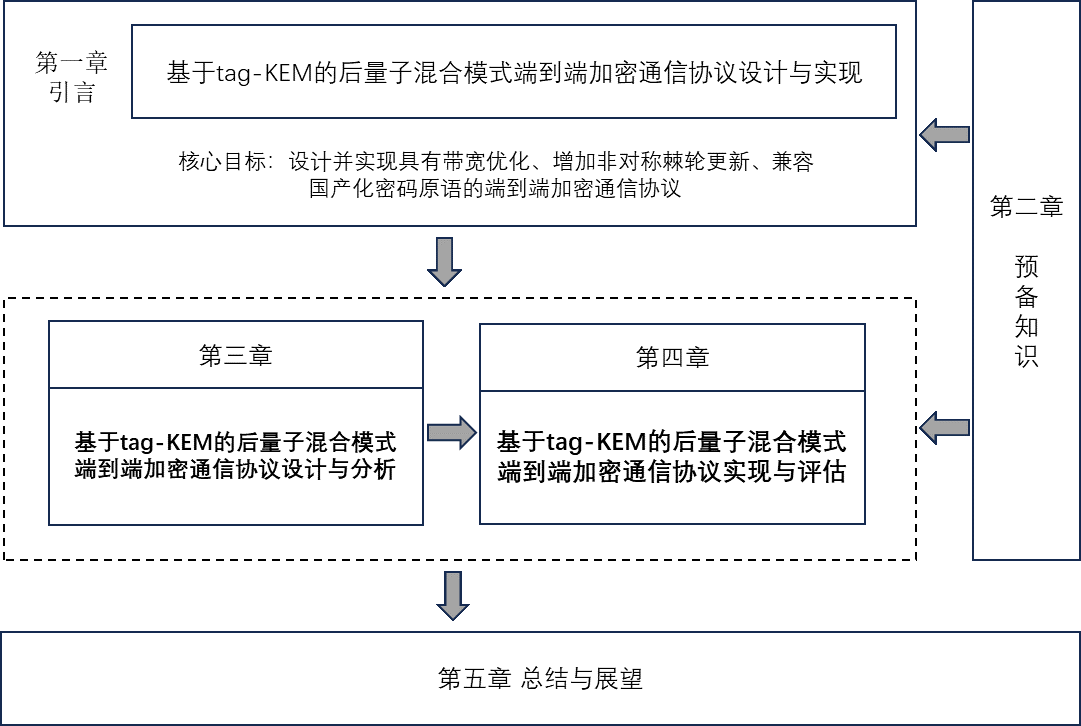
\includegraphics[width=\linewidth]{Img/章节安排.png} 
    \caption{章节安排}
    \label{fig:schedule}
  
  \label{fig:schedule}
\end{figure}


第一章说明背景，研究现状以及存在的问题，确定本工作的具体内容；

第二章介绍必要的知识点和相关技术；

第三章是本工作的核心内容，现有方案（pqxdh、pq3）对比、算法流程（一些非标准算法）；

包括方案设计（可以兼容）+本工作的安全模型、安全性分析、具体实现、对话效果（测试）；

第四章是具体的实现以及实验测试结果，实验测试；

第五章是总结本工作的贡献、存在不足以及展望。


